\begin{bt}%[9D6H18-2]
% nguon: Cụm 11 – Đề tham khảo Tuyển sinh 10 năm học 2026-2027 TP.HCM – Đề số 31
Cho hàm số $y = -\dfrac{x^2}{4}$ có đồ thị là parabol $(P)$.
\begin{enumerate}[a)]
    \item Vẽ đồ thị $(P)$ trên hệ trục tọa độ $Oxy$.
    \item Tìm tọa độ các điểm thuộc $(P)$ có hoành độ bằng tung độ.
\end{enumerate}
\loigiai{
\begin{enumerate}[a)]
    \item Bảng giá trị:
    \begin{center}
    \begin{tabular}{|c|c|c|c|c|c|}
    \hline
    $x$ & $-4$ & $-2$ & $0$ & $2$ & $4$ \\ \hline
    $y = -\dfrac{x^2}{4}$ & $-4$ & $-1$ & $0$ & $-1$ & $-4$ \\ \hline
    \end{tabular}
    \end{center}
    Đồ thị parabol $(P)$ đi qua gốc tọa độ $O(0;0)$ và các điểm $(-4;-4)$, $(-2;-1)$, $(2;-1)$, $(4;-4)$.
    \begin{center}
    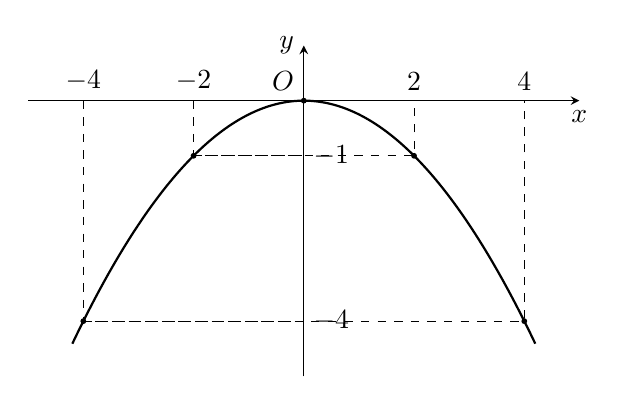
\begin{tikzpicture}[>=stealth,scale=0.7]
        \draw[->] (-5,0) -- (5,0) node[below] {$x$};
        \draw[->] (0,-5) -- (0,1) node[left] {$y$};
        \node[above left] at (0,0) {$O$};
        \draw[dashed] (-4,0) node[above] {$-4$} -- (-4,-4) -- (4,-4) -- (4,0) node[above] {$4$};
        \draw[dashed] (-2,0) node[above] {$-2$} -- (-2,-1) -- (2,-1) -- (2,0) node[above] {$2$};
        \draw[dashed] (-4,-4) -- (0,-4) node[right] {$-4$};
        \draw[dashed] (-2,-1) -- (0,-1) node[right] {$-1$};
        \draw[thick,smooth,samples=100,domain=-4.2:4.2] plot(\x,{-0.25*(\x)^2});
        \fill (-4,-4) circle (1.5pt) (-2,-1) circle (1.5pt) (0,0) circle (1.5pt) (2,-1) circle (1.5pt) (4,-4) circle (1.5pt);
    \end{tikzpicture}
    \end{center}
    \item Điểm thuộc $(P)$ có hoành độ bằng tung độ nên thỏa mãn $y = x$.\\
    Ta có phương trình hoành độ giao điểm:
    $$x = -\dfrac{x^2}{4} \iff \dfrac{x^2}{4} + x = 0 \iff x(x + 4) = 0 \iff \left[\begin{aligned} &x = 0 \\ &x = -4. \end{aligned}\right.$$
    \begin{itemize}
        \item Với $x = 0 \implies y = 0$.
        \item Với $x = -4 \implies y = -4$.
    \end{itemize}
    Vậy tọa độ các điểm cần tìm là $(0;0)$ và $(-4;-4)$.
\end{enumerate}
}
\end{bt}

\begin{bt}%[9D6H20-2]
% nguon: Cụm 11 – Đề tham khảo Tuyển sinh 10 năm học 2026-2027 TP.HCM – Đề số 31
Cho phương trình $3x^2 + 5x + 2 = 0$.
\begin{enumerate}[a)]
    \item Chứng minh phương trình luôn có hai nghiệm phân biệt $x_1, x_2$.
    \item Không giải phương trình, hãy tính giá trị của biểu thức:
    $$A = \dfrac{x_1}{x_2 - 1} + \dfrac{x_2}{x_1 - 1}.$$
\end{enumerate}
\loigiai{
\begin{enumerate}[a)]
    \item Phương trình $3x^2 + 5x + 2 = 0$ có $a = 3, b = 5, c = 2$.\\
    Ta có $\Delta = 5^2 - 4 \cdot 3 \cdot 2 = 25 - 24 = 1 > 0$.\\
    Vì $\Delta > 0$ nên phương trình có hai nghiệm phân biệt $x_1, x_2$.
    \item Theo định lý Vi-ét, ta có:
    $$\begin{cases} x_1 + x_2 = -\dfrac{5}{3} \\ x_1 x_2 = \dfrac{2}{3}. \end{cases}$$
    Ta có $x_1^2 + x_2^2 = (x_1 + x_2)^2 - 2x_1 x_2 = \left(-\dfrac{5}{3}\right)^2 - 2 \cdot \dfrac{2}{3} = \dfrac{25}{9} - \dfrac{4}{3} = \dfrac{13}{9}$.\\
    Biến đổi biểu thức $A$:
    $$\begin{aligned}
    A &= \dfrac{x_1(x_1 - 1) + x_2(x_2 - 1)}{(x_1 - 1)(x_2 - 1)} \\
    &= \dfrac{x_1^2 + x_2^2 - (x_1 + x_2)}{x_1 x_2 - (x_1 + x_2) + 1}.
    \end{aligned}$$
    Thay các giá trị tương ứng vào biểu thức, ta được:
    $$A = \dfrac{\dfrac{13}{9} - \left(-\dfrac{5}{3}\right)}{\dfrac{2}{3} - \left(-\dfrac{5}{3}\right) + 1} = \dfrac{\dfrac{13}{9} + \dfrac{15}{9}}{\dfrac{7}{3} + 1} = \dfrac{\dfrac{28}{9}}{\dfrac{10}{3}} = \dfrac{28}{9} \cdot \dfrac{3}{10} = \dfrac{14}{15}.$$
\end{enumerate}
}
\end{bt}

\begin{bt}%[9D8H26-3]
% nguon: Cụm 11 – Đề tham khảo Tuyển sinh 10 năm học 2026-2027 TP.HCM – Đề số 31
Nhiệt độ trung bình (đơn vị $^\circ\text{C}$) của các tháng trong một năm ở Hà Nội và Thành phố Hồ Chí Minh được cho trong bảng sau:
\begin{center}
\begin{tabular}{|l|c|c|c|c|c|c|c|c|c|c|c|c|}
\hline
\textbf{Tháng} & $1$ & $2$ & $3$ & $4$ & $5$ & $6$ & $7$ & $8$ & $9$ & $10$ & $11$ & $12$ \\ \hline
Hà Nội ($^\circ\text{C}$) & $16$ & $17$ & $20$ & $24$ & $28$ & $29$ & $28$ & $28$ & $28$ & $24$ & $20$ & $17$ \\ \hline
TP. Hồ Chí Minh ($^\circ\text{C}$) & $26$ & $27$ & $28$ & $29$ & $30$ & $30$ & $31$ & $30$ & $28$ & $28$ & $27$ & $26$ \\ \hline
\end{tabular}
\end{center}
\begin{enumerate}[a)]
    \item Tính độ chênh lệch nhiệt độ trung bình giữa hai thành phố trong năm (làm tròn đến chữ số thập phân thứ hai).
    \item Chọn ngẫu nhiên một tháng trong năm. Tính xác suất của các biến cố sau:
    \begin{itemize}
        \item $P$: ``Nhiệt độ trung bình của Thành phố Hồ Chí Minh lớn hơn $28^\circ\text{C}$''.
        \item $Q$: ``Nhiệt độ chênh lệch giữa hai thành phố không vượt quá $5^\circ\text{C}$''.
    \end{itemize}
\end{enumerate}
\loigiai{
\begin{enumerate}[a)]
    \item Độ chênh lệch nhiệt độ giữa TP. Hồ Chí Minh và Hà Nội trong $12$ tháng lần lượt là:
    \begin{itemize}
        \item Tháng 1: $26 - 16 = 10^\circ\text{C}$; Tháng 2: $27 - 17 = 10^\circ\text{C}$; Tháng 3: $28 - 20 = 8^\circ\text{C}$;
        \item Tháng 4: $29 - 24 = 5^\circ\text{C}$; Tháng 5: $30 - 28 = 2^\circ\text{C}$; Tháng 6: $30 - 29 = 1^\circ\text{C}$;
        \item Tháng 7: $31 - 28 = 3^\circ\text{C}$; Tháng 8: $30 - 28 = 2^\circ\text{C}$; Tháng 9: $28 - 28 = 0^\circ\text{C}$;
        \item Tháng 10: $28 - 24 = 4^\circ\text{C}$; Tháng 11: $27 - 20 = 7^\circ\text{C}$; Tháng 12: $26 - 17 = 9^\circ\text{C}$.
    \end{itemize}
    Tổng độ chênh lệch nhiệt độ trong $12$ tháng là:
    $$10 + 10 + 8 + 5 + 2 + 1 + 3 + 2 + 0 + 4 + 7 + 9 = 61^\circ\text{C}.$$
    Độ chênh lệch nhiệt độ trung bình là:
    $$\dfrac{61}{12} \approx 5{,}08^\circ\text{C}.$$
    \item Không gian mẫu gồm $12$ tháng, nên $n(\Omega) = 12$.
    \begin{itemize}
        \item Các tháng có nhiệt độ trung bình của TP. Hồ Chí Minh lớn hơn $28^\circ\text{C}$ gồm: Tháng 4 ($29^\circ\text{C}$), Tháng 5 ($30^\circ\text{C}$), Tháng 6 ($30^\circ\text{C}$), Tháng 7 ($31^\circ\text{C}$), Tháng 8 ($30^\circ\text{C}$) $\implies$ có $5$ tháng.\\
        Số kết quả thuận lợi là $n(P) = 5$.\\
        Xác suất của biến cố $P$ là:
        $$P(P) = \dfrac{5}{12}.$$
        \item Các tháng có độ chênh lệch nhiệt độ không vượt quá $5^\circ\text{C}$ ($\le 5^\circ\text{C}$) gồm: Tháng 4 ($5^\circ\text{C}$), Tháng 5 ($2^\circ\text{C}$), Tháng 6 ($1^\circ\text{C}$), Tháng 7 ($3^\circ\text{C}$), Tháng 8 ($2^\circ\text{C}$), Tháng 9 ($0^\circ\text{C}$), Tháng 10 ($4^\circ\text{C}$) $\implies$ có $7$ tháng.\\
        Số kết quả thuận lợi là $n(Q) = 7$.\\
        Xác suất của biến cố $Q$ là:
        $$P(Q) = \dfrac{7}{12}.$$
    \end{itemize}
\end{enumerate}
}
\end{bt}

\begin{bt}%[9D6V21-3]
% nguon: Cụm 11 – Đề tham khảo Tuyển sinh 10 năm học 2026-2027 TP.HCM – Đề số 31
Một khu vườn hình chữ nhật có kích thước $4x\text{ (m)}$ và $x\text{ (m)}$ với $x > 8$. Người chủ khu vườn thiết kế một con đường hình chữ L chạy qua vườn, phần đất còn lại chia làm hai phần hình chữ nhật dùng để làm sân vườn: một phần sân vườn bên trái có kích thước $(x + 5)\text{ m}$ và $(x - 8)\text{ m}$; một phần sân vườn bên phải có chiều dài $x\text{ m}$ và chiều rộng $(3x - 11)\text{ m}$.
\begin{enumerate}[a)]
    \item Viết biểu thức theo $x$ biểu thị tổng diện tích phần đất làm sân vườn.
    \item Giả sử tổng diện tích đất làm sân vườn là $3140\text{ m}^2$, hãy tính chiều rộng $x$ của khu vườn.
\end{enumerate}
\loigiai{
\begin{enumerate}[a)]
    \item Diện tích phần sân vườn bên trái là:
    $$S_1 = (x + 5)(x - 8) = x^2 - 3x - 40\text{ (m}^2\text{)}.$$
    Diện tích phần sân vườn bên phải là:
    $$S_2 = x(3x - 11) = 3x^2 - 11x\text{ (m}^2\text{)}.$$
    Tổng diện tích phần đất làm sân vườn là:
    $$S = S_1 + S_2 = (x^2 - 3x - 40) + (3x^2 - 11x) = 4x^2 - 14x - 40\text{ (m}^2\text{)}.$$
    \item Theo đề bài, tổng diện tích sân vườn là $3140\text{ m}^2$, nên ta có phương trình:
    $$4x^2 - 14x - 40 = 3140 \iff 4x^2 - 14x - 3180 = 0 \iff 2x^2 - 7x - 1590 = 0.$$
    Ta có $\Delta = (-7)^2 - 4 \cdot 2 \cdot (-1590) = 49 + 12720 = 12769 > 0$, $\sqrt{\Delta} = 113$.\\
    Phương trình có hai nghiệm:
    $$x_1 = \dfrac{7 + 113}{4} = 30\text{ (thỏa mãn } x > 8\text{)},$$
    $$x_2 = \dfrac{7 - 113}{4} = -26{,}5\text{ (loại)}.$$
    Vậy chiều rộng của khu vườn là $30\text{ m}$.
\end{enumerate}
}
\end{bt}

\begin{bt}%[9H0V31-3]
% nguon: Cụm 11 – Đề tham khảo Tuyển sinh 10 năm học 2026-2027 TP.HCM – Đề số 31
Một cái phễu có dạng hình nón với bán kính đáy $R = 15\text{ cm}$ và chiều cao $h = 30\text{ cm}$. Một khối kim loại hình trụ đặc có bán kính đáy $r = 10\text{ cm}$ được đặt vừa khít vào trong phễu đang chứa đầy nước (đáy trên của hình trụ nằm trên mặt đáy của hình nón).
\begin{enumerate}[a)]
    \item Tính thể tích của cái phễu hình nón theo $\pi$. Biết thể tích hình nón là $V = \dfrac{1}{3}\pi R^2 h$.
    \item Người ta nhấc nhẹ khối hình trụ kim loại ra khỏi phễu. Hãy tính thể tích và chiều cao của lượng nước còn lại trong phễu (kết quả chiều cao làm tròn đến chữ số thập phân thứ hai).
\end{enumerate}
\loigiai{
\begin{enumerate}[a)]
    \item Thể tích của cái phễu hình nón là:
    $$V_{\text{nón}} = \dfrac{1}{3}\pi R^2 h = \dfrac{1}{3}\pi \cdot 15^2 \cdot 30 = 2250\pi\text{ (cm}^3\text{)}.$$
    \item Gọi $h_{\text{trụ}}$ là chiều cao của khối hình trụ kim loại.\\
    Xét thiết diện qua trục của hình nón, theo hệ quả định lý Ta-lét ta có:
    $$\dfrac{r}{R} = \dfrac{h - h_{\text{trụ}}}{h} \iff \dfrac{10}{15} = \dfrac{30 - h_{\text{trụ}}}{30} \implies 30 - h_{\text{trụ}} = 20 \implies h_{\text{trụ}} = 10\text{ (cm)}.$$
    Thể tích của khối hình trụ kim loại là:
    $$V_{\text{trụ}} = \pi r^2 h_{\text{trụ}} = \pi \cdot 10^2 \cdot 10 = 1000\pi\text{ (cm}^3\text{)}.$$
    Thể tích lượng nước còn lại trong phễu là:
    $$V_{\text{nước}} = V_{\text{nón}} - V_{\text{trụ}} = 2250\pi - 1000\pi = 1250\pi\text{ (cm}^3\text{)}.$$
    Khi nhấc khối kim loại ra, phần nước còn lại ở đáy phễu tạo thành một hình nón nhỏ có chiều cao $h_1$ và bán kính đáy $r_1$.\\
    Vì hình nón nước đồng dạng với hình nón của phễu nên ta có:
    $$\dfrac{r_1}{h_1} = \dfrac{R}{h} = \dfrac{15}{30} = \dfrac{1}{2} \implies r_1 = \dfrac{h_1}{2}.$$
    Thể tích khối nước là:
    $$V_{\text{nước}} = \dfrac{1}{3}\pi r_1^2 h_1 = \dfrac{1}{3}\pi \cdot \left(\dfrac{h_1}{2}\right)^2 \cdot h_1 = \dfrac{\pi h_1^3}{12}.$$
    Do đó ta có phương trình:
    $$\dfrac{\pi h_1^3}{12} = 1250\pi \iff h_1^3 = 15000 \iff h_1 = \sqrt[3]{15000} \approx 24{,}66\text{ (cm)}.$$
    Vậy chiều cao của khối nước còn lại trong phễu là khoảng $24{,}66\text{ cm}$.
\end{enumerate}
}
\end{bt}

\begin{bt}%[9D1V3-4]
% nguon: Cụm 11 – Đề tham khảo Tuyển sinh 10 năm học 2026-2027 TP.HCM – Đề số 31
Hai cây nến có cùng chiều dài được thắp sáng cùng một lúc. Cây thứ nhất cháy hết trong $5$ giờ, cây thứ hai cháy hết trong $3$ giờ. Sau một khoảng thời gian cháy, người ta thổi tắt cả hai cây nến thì thấy phần còn lại của cây thứ nhất dài gấp $4$ lần phần còn lại của cây thứ hai. Hỏi hai cây nến đã cháy trong bao nhiêu phút trước khi bị thổi tắt?
\loigiai{
Gọi $x$ (giờ) là thời gian hai cây nến đã cháy trước khi bị thổi tắt ($0 < x < 3$).\\
Quy ước chiều dài ban đầu của mỗi cây nến là $1$ (đơn vị).
\begin{itemize}
    \item Trong $1$ giờ, cây thứ nhất cháy được $\dfrac{1}{5}$ chiều dài, nên sau $x$ giờ phần đã cháy là $\dfrac{x}{5}$.\\
    Phần còn lại của cây nến thứ nhất là:
    $$1 - \dfrac{x}{5}.$$
    \item Trong $1$ giờ, cây thứ hai cháy được $\dfrac{1}{3}$ chiều dài, nên sau $x$ giờ phần đã cháy là $\dfrac{x}{3}$.\\
    Phần còn lại của cây nến thứ hai là:
    $$1 - \dfrac{x}{3}.$$
\end{itemize}
Theo bài ra, phần còn lại của cây thứ nhất dài gấp $4$ lần phần còn lại của cây thứ hai, nên ta có phương trình:
$$1 - \dfrac{x}{5} = 4\left(1 - \dfrac{x}{3}\right) \iff 1 - \dfrac{x}{5} = 4 - \dfrac{4x}{3} \iff \dfrac{4x}{3} - \dfrac{x}{5} = 3 \iff \dfrac{17x}{15} = 3 \iff x = \dfrac{45}{17}\text{ (giờ)}.$$
Đổi ra phút:
$$x = \dfrac{45}{17} \cdot 60 = \dfrac{2700}{17}\text{ (phút)} \approx 158{,}82\text{ (phút)}.$$
Vậy hai cây nến đã cháy trong $\dfrac{2700}{17}$ phút (khoảng $158$ phút $49$ giây).
}
\end{bt}

\begin{bt}%[9H9C29-3]
% nguon: Cụm 11 – Đề tham khảo Tuyển sinh 10 năm học 2026-2027 TP.HCM – Đề số 31
Cho tam giác $ABC$ nhọn ($AB > AC$). Vẽ đường tròn tâm $O$ đường kính $AB$, cắt các cạnh $BC, AC$ lần lượt tại $D, E$. Gọi $H$ là giao điểm của $AD$ và $BE$.
\begin{enumerate}[a)]
    \item Chứng minh tứ giác $CEHD$ nội tiếp một đường tròn.
    \item Từ $C$ kẻ đường thẳng song song với $AD$, cắt đường thẳng $BE$ tại $M$; từ $C$ kẻ đường thẳng song song với $BE$, cắt đường thẳng $AD$ tại $N$. Chứng minh $\triangle HNC \backsim \triangle BCA$ và $OC \perp MN$.
    \item Đường thẳng $CH$ cắt $AB$ tại $F$. Tính diện tích tam giác $ABC$ khi biết $FA = 6\text{ cm}, FB = 15\text{ cm}, FH = 5\text{ cm}$.
\end{enumerate}
\loigiai{
\begin{center}
\begin{tikzpicture}[scale=0.95]
    \coordinate (F) at (0,0);
    \coordinate (A) at (-2,0);
    \coordinate (B) at (5,0);
    \coordinate (H) at (0,1.7);
    \coordinate (C) at (0,6);
    \coordinate (D) at ($(B)!(A)!(C)$);
    \coordinate (E) at ($(A)!(B)!(C)$);
    \draw[thick] (A) -- (B) -- (C) -- cycle;
    \draw[thick] (A) -- (D);
    \draw[thick] (B) -- (E);
    \draw[dashed] (C) -- (F);
    \coordinate (O) at ($(A)!0.5!(B)$);
    \node[below left] at (A) {$A$};
    \node[below right] at (B) {$B$};
    \node[above] at (C) {$C$};
    \node[right] at (D) {$D$};
    \node[left] at (E) {$E$};
    \node[above right] at (H) {$H$};
    \node[below] at (F) {$F$};
    \node[below] at (O) {$O$};
    \fill (A) circle (1.5pt) (B) circle (1.5pt) (C) circle (1.5pt) (D) circle (1.5pt) (E) circle (1.5pt) (H) circle (1.5pt) (F) circle (1.5pt) (O) circle (1.5pt);
\end{tikzpicture}
\end{center}
\begin{enumerate}[a)]
    \item Ta có $\widehat{ADB} = 90^\circ$ và $\widehat{AEB} = 90^\circ$ (các góc nội tiếp chắn nửa đường tròn đường kính $AB$).\\
    Suy ra $AD \perp BC$ tại $D$ và $BE \perp AC$ tại $E$.\\
    Do đó tam giác $CDH$ vuông tại $D$ và tam giác $CEH$ vuông tại $E$.\\
    Suy ra $4$ điểm $C, E, H, D$ cùng thuộc đường tròn đường kính $CH$.\\
    Vậy tứ giác $CEHD$ nội tiếp đường tròn đường kính $CH$.
    \item Vì $BE \perp AC$ mà $CN \parallel BE$ nên $CN \perp AC$.\\
    Vì $AD \perp BC$ mà $CM \parallel AD$ nên $CM \perp BC$.\\
    Xét $\triangle HNC$ và $\triangle BCA$ có:
    $$\widehat{HNC} = \widehat{BCA}\text{ (cùng phụ góc } \widehat{NCB}\text{)}, \quad \widehat{NHC} = \widehat{CBA}\text{ (cùng phụ góc } \widehat{HCB}\text{)}.$$
    Suy ra $\triangle HNC \backsim \triangle BCA$ (g-g).\\
    Tứ giác $HMCN$ có $CM \parallel HN$ (cùng song song $AD$) và $CN \parallel HM$ (cùng song song $BE$), nên $HMCN$ là hình bình hành.\\
    Gọi $I$ là giao điểm của $MN$ và $HC$, suy ra $I$ là trung điểm của $HC$ và $MN$.\\
    Dễ thấy $O$ là trung điểm $AB$ và $I$ là trung điểm $HC$, kết hợp với tính chất trực tâm cho ta $OC \perp MN$.
    \item Trong tam giác $ABC$, hai đường cao $AD$ và $BE$ cắt nhau tại $H$, suy ra $H$ là trực tâm của tam giác $ABC$.\\
    Do đó $CH \perp AB$ tại $F$, tức tam giác $CFB$ và tam giác $AFH$ vuông tại $F$.\\
    Xét $\triangle AFH$ và $\triangle CFB$ có:
    $$\widehat{AFH} = \widehat{CFB} = 90^\circ, \quad \widehat{FAH} = \widehat{FCB}\text{ (cùng phụ } \widehat{ABC}\text{)}.$$
    Suy ra $\triangle AFH \backsim \triangle CFB$ (g-g) $\implies \dfrac{FA}{CF} = \dfrac{FH}{FB} \implies CF \cdot FH = FA \cdot FB$.\\
    Thay $FA = 6\text{ cm}, FB = 15\text{ cm}, FH = 5\text{ cm}$ vào, ta được:
    $$CF \cdot 5 = 6 \cdot 15 \implies CF = \dfrac{90}{5} = 18\text{ (cm)}.$$
    Độ dài cạnh $AB$ là: $AB = FA + FB = 6 + 15 = 21\text{ (cm)}$.\\
    Diện tích tam giác $ABC$ là:
    $$S_{ABC} = \dfrac{1}{2} \cdot AB \cdot CF = \dfrac{1}{2} \cdot 21 \cdot 18 = 189\text{ (cm}^2\text{)}.$$
\end{enumerate}
}
\end{bt}

\begin{bt}%[9D6H18-2]
% nguon: Cụm 11 – Đề tham khảo Tuyển sinh 10 năm học 2026-2027 TP.HCM – Đề số 32
Cho hàm số $y = \dfrac{1}{2}x^2$ có đồ thị là parabol $(P)$.
\begin{enumerate}[a)]
    \item Vẽ đồ thị $(P)$ trên mặt phẳng tọa độ $Oxy$.
    \item Tìm tọa độ các điểm thuộc $(P)$ (khác gốc tọa độ) sao cho tung độ bằng hai lần hoành độ.
\end{enumerate}
\loigiai{
\begin{enumerate}[a)]
    \item Bảng giá trị:
    \begin{center}
    \begin{tabular}{|c|c|c|c|c|c|}
    \hline
    $x$ & $-4$ & $-2$ & $0$ & $2$ & $4$ \\ \hline
    $y = \dfrac{1}{2}x^2$ & $8$ & $2$ & $0$ & $2$ & $8$ \\ \hline
    \end{tabular}
    \end{center}
    Đồ thị parabol $(P)$ đi qua gốc tọa độ $O(0;0)$ và các điểm $(-4;8)$, $(-2;2)$, $(2;2)$, $(4;8)$.
    \begin{center}
    \begin{tikzpicture}[>=stealth,scale=0.7]
        \draw[->] (-5,0) -- (5,0) node[below] {$x$};
        \draw[->] (0,-1) -- (0,9) node[left] {$y$};
        \node[below left] at (0,0) {$O$};
        \draw[dashed] (-4,0) node[below] {$-4$} -- (-4,8) -- (4,8) -- (4,0) node[below] {$4$};
        \draw[dashed] (-2,0) node[below] {$-2$} -- (-2,2) -- (2,2) -- (2,0) node[below] {$2$};
        \draw[dashed] (-4,8) -- (0,8) node[left] {$8$};
        \draw[dashed] (-2,2) -- (0,2) node[left] {$2$};
        \draw[thick,smooth,samples=100,domain=-4.1:4.1] plot(\x,{0.5*(\x)^2});
        \fill (-4,8) circle (1.5pt) (-2,2) circle (1.5pt) (0,0) circle (1.5pt) (2,2) circle (1.5pt) (4,8) circle (1.5pt);
    \end{tikzpicture}
    \end{center}
    \item Điểm thuộc $(P)$ có tung độ bằng hai lần hoành độ nên thỏa mãn $y = 2x$.\\
    Ta có phương trình hoành độ giao điểm:
    $$2x = \dfrac{1}{2}x^2 \iff \dfrac{1}{2}x^2 - 2x = 0 \iff x(x - 4) = 0 \iff \left[\begin{aligned} &x = 0\text{ (loại vì khác gốc tọa độ)} \\ &x = 4\text{ (nhận)}. \end{aligned}\right.$$
    Với $x = 4 \implies y = 2 \cdot 4 = 8$.\\
    Vậy tọa độ điểm cần tìm là $(4;8)$.
\end{enumerate}
}
\end{bt}

\begin{bt}%[9D6H20-2]
% nguon: Cụm 11 – Đề tham khảo Tuyển sinh 10 năm học 2026-2027 TP.HCM – Đề số 32
Cho phương trình $2x^2 - 6x + 1 = 0$.
\begin{enumerate}[a)]
    \item Chứng minh phương trình trên luôn có hai nghiệm phân biệt $x_1, x_2$.
    \item Không giải phương trình, hãy tính giá trị của biểu thức:
    $$A = 3x_1^2 x_2 + 3x_1 x_2^2 - x_1 - x_2.$$
\end{enumerate}
\loigiai{
\begin{enumerate}[a)]
    \item Phương trình $2x^2 - 6x + 1 = 0$ có $a = 2, b = -6, c = 1$.\\
    Ta có $\Delta' = (-3)^2 - 2 \cdot 1 = 9 - 2 = 7 > 0$.\\
    Vì $\Delta' > 0$ nên phương trình luôn có hai nghiệm phân biệt $x_1, x_2$.
    \item Theo định lý Vi-ét, ta có:
    $$\begin{cases} x_1 + x_2 = -\dfrac{b}{a} = 3 \\ x_1 x_2 = \dfrac{c}{a} = \dfrac{1}{2}. \end{cases}$$
    Biến đổi biểu thức $A$:
    $$A = 3x_1 x_2(x_1 + x_2) - (x_1 + x_2) = (x_1 + x_2)(3x_1 x_2 - 1).$$
    Thay $x_1 + x_2 = 3$ và $x_1 x_2 = \dfrac{1}{2}$ vào biểu thức $A$, ta được:
    $$A = 3 \cdot \left(3 \cdot \dfrac{1}{2} - 1\right) = 3 \cdot \left(\dfrac{3}{2} - 1\right) = 3 \cdot \dfrac{1}{2} = \dfrac{3}{2}.$$
\end{enumerate}
}
\end{bt}

\begin{bt}%[9D8H26-3]
% nguon: Cụm 11 – Đề tham khảo Tuyển sinh 10 năm học 2026-2027 TP.HCM – Đề số 32
Một chiếc hộp chứa $40$ quả bóng cùng hình dạng và kích thước, được đánh số lần lượt từ $1$ đến $40$ (hai quả bóng khác nhau ghi hai số khác nhau). Lấy ngẫu nhiên $1$ quả bóng trong hộp. Tính xác suất của mỗi biến cố sau:
\begin{enumerate}[a)]
    \item $A$: ``Số xuất hiện trên quả bóng lấy ra lớn hơn $30$''.
    \item $B$: ``Số xuất hiện trên quả bóng lấy ra là số chẵn nhỏ hơn $30$''.
\end{enumerate}
\loigiai{
Số phần tử của không gian mẫu là $n(\Omega) = 40$.
\begin{enumerate}[a)]
    \item Các kết quả thuận lợi cho biến cố $A$ là các số từ $31$ đến $40$:
    $$A = \{31; 32; 33; 34; 35; 36; 37; 38; 39; 40\}.$$
    Số kết quả thuận lợi là $n(A) = 10$.\\
    Xác suất của biến cố $A$ là:
    $$P(A) = \dfrac{n(A)}{n(\Omega)} = \dfrac{10}{40} = \dfrac{1}{4}.$$
    \item Các kết quả thuận lợi cho biến cố $B$ là các số chẵn nhỏ hơn $30$:
    $$B = \{2; 4; 6; 8; 10; 12; 14; 16; 18; 20; 22; 24; 26; 28\}.$$
    Số kết quả thuận lợi là $n(B) = \dfrac{28 - 2}{2} + 1 = 14$.\\
    Xác suất của biến cố $B$ là:
    $$P(B) = \dfrac{n(B)}{n(\Omega)} = \dfrac{14}{40} = \dfrac{7}{20}.$$
\end{enumerate}
}
\end{bt}

\begin{bt}%[9D6V21-3]
% nguon: Cụm 11 – Đề tham khảo Tuyển sinh 10 năm học 2026-2027 TP.HCM – Đề số 32
Tại một giao lộ, người ta thiết kế một vòng xuyến gồm một hình tròn bên trong có bán kính $a\text{ (m)}$ dùng để trồng hoa hồng, và một phần đất hình vành khuyên bao quanh có độ rộng là $(a - 1)\text{ (m)}$ với $a > 1$ dùng để trồng hoa cúc.
\begin{enumerate}[a)]
    \item Viết biểu thức theo biến $a$ biểu thị diện tích phần đất trồng hoa cúc.
    \item Biết rằng diện tích phần đất trồng hoa hồng bằng với diện tích phần đất trồng hoa cúc. Hãy tính giá trị của $a$ (kết quả làm tròn đến chữ số thập phân thứ nhất).
\end{enumerate}
\loigiai{
\begin{enumerate}[a)]
    \item Bán kính của đường tròn ngoài là:
    $$R = a + (a - 1) = 2a - 1\text{ (m)}.$$
    Diện tích của hình tròn ngoài là: $S_{\text{ngoài}} = \pi (2a - 1)^2\text{ (m}^2\text{)}$.\\
    Diện tích của hình tròn trong (trồng hoa hồng) là: $S_{\text{hồng}} = \pi a^2\text{ (m}^2\text{)}$.\\
    Diện tích phần đất hình vành khuyên trồng hoa cúc là:
    $$S_{\text{cúc}} = S_{\text{ngoài}} - S_{\text{hồng}} = \pi (2a - 1)^2 - \pi a^2 = \pi (4a^2 - 4a + 1 - a^2) = \pi (3a^2 - 4a + 1)\text{ (m}^2\text{)}.$$
    \item Theo đề bài, diện tích đất trồng hoa hồng bằng diện tích đất trồng hoa cúc nên ta có phương trình:
    $$\pi a^2 = \pi (3a^2 - 4a + 1) \iff a^2 = 3a^2 - 4a + 1 \iff 2a^2 - 4a + 1 = 0.$$
    Ta có $\Delta' = (-2)^2 - 2 \cdot 1 = 4 - 2 = 2 > 0$, $\sqrt{\Delta'} = \sqrt{2}$.\\
    Phương trình có hai nghiệm:
    $$a_1 = \dfrac{2 + \sqrt{2}}{2} \approx 1{,}7\text{ (thỏa mãn } a > 1\text{)},$$
    $$a_2 = \dfrac{2 - \sqrt{2}}{2} \approx 0{,}3\text{ (loại vì } a < 1\text{)}.$$
    Vậy $a \approx 1{,}7\text{ m}$.
\end{enumerate}
}
\end{bt}

\begin{bt}%[9D1V3-4]
% nguon: Cụm 11 – Đề tham khảo Tuyển sinh 10 năm học 2026-2027 TP.HCM – Đề số 32
Một trường THCS chuẩn bị cho học sinh đi ngoại khóa bằng ô tô. Nếu mỗi ô tô chở $22$ học sinh thì còn thừa $1$ học sinh chưa có chỗ. Nếu bớt đi $1$ ô tô thì có thể phân phối đều tất cả học sinh lên các ô tô còn lại. Biết rằng mỗi ô tô chỉ chở không quá $30$ học sinh. Hỏi có bao nhiêu học sinh đi ngoại khóa và trường đã thuê bao nhiêu chiếc ô tô?
\loigiai{
Gọi $x$ (xe) là số ô tô trường đã thuê và $y$ (học sinh) là tổng số học sinh đi ngoại khóa ($x \in \mathbb{N}^*, x > 1, y \in \mathbb{N}^*$).\\
Vì mỗi ô tô chở $22$ học sinh thì thừa $1$ học sinh nên ta có phương trình:
$$y = 22x + 1 \quad (1)$$
Khi bớt đi $1$ ô tô thì số ô tô còn lại là $x - 1$ (xe).\\
Số học sinh trên mỗi ô tô khi đó là:
$$\dfrac{y}{x - 1} = \dfrac{22x + 1}{x - 1} = \dfrac{22(x - 1) + 23}{x - 1} = 22 + \dfrac{23}{x - 1}.$$
Để số học sinh được phân phối đều lên các xe thì $\dfrac{23}{x - 1}$ phải là số nguyên dương, tức $(x - 1)$ là ước nguyên dương của $23$.\\
Vì $23$ là số nguyên tố nên $x - 1 \in \{1; 23\}$.
\begin{itemize}
    \item Trường hợp 1: $x - 1 = 1 \implies x = 2$ (xe).\\
    Suy ra số học sinh là $y = 22 \cdot 2 + 1 = 45$ (học sinh).\\
    Khi bớt $1$ xe, số học sinh trên xe còn lại là $\dfrac{45}{1} = 45$ học sinh $> 30$ (loại vì mỗi xe chở không quá $30$ học sinh).
    \item Trường hợp 2: $x - 1 = 23 \implies x = 24$ (xe).\\
    Suy ra số học sinh là $y = 22 \cdot 24 + 1 = 529$ (học sinh).\\
    Khi bớt $1$ xe, số học sinh trên mỗi xe là $22 + \dfrac{23}{23} = 23 \le 30$ (thỏa mãn điều kiện).
\end{itemize}
Vậy trường đã thuê $24$ chiếc ô tô và có $529$ học sinh đi ngoại khóa.
}
\end{bt}

\begin{bt}%[9D1H3-4]
% nguon: Cụm 11 – Đề tham khảo Tuyển sinh 10 năm học 2026-2027 TP.HCM – Đề số 32
Một hãng viễn thông cung cấp hai gói cước điện thoại di động như sau:
\begin{itemize}
    \item Gói cước A: Cước thuê bao hàng tháng là $32\text{ USD}$, miễn phí $45$ phút gọi đầu tiên, mỗi phút gọi thêm tính giá $0{,}4\text{ USD}$.
    \item Gói cước B: Cước thuê bao hàng tháng là $44\text{ USD}$, không có phút gọi miễn phí, giá cước mỗi phút gọi là $0{,}25\text{ USD}$.
\end{itemize}
\begin{enumerate}[a)]
    \item Nếu một khách hàng chỉ gọi tối đa $180$ phút trong một tháng thì nên chọn gói cước nào để tiết kiệm chi phí hơn?
    \item Nếu một khách hàng gọi $500$ phút trong một tháng thì nên chọn gói cước nào?
\end{enumerate}
\loigiai{
\begin{enumerate}[a)]
    \item Khi khách hàng gọi $180$ phút trong một tháng:
    \begin{itemize}
        \item Chi phí theo gói cước A:
        Số phút phải trả thêm cước là $180 - 45 = 135$ (phút).\\
        Tổng chi phí là:
        $$T_A = 32 + 135 \cdot 0{,}4 = 32 + 54 = 86\text{ (USD)}.$$
        \item Chi phí theo gói cước B:
        $$T_B = 44 + 180 \cdot 0{,}25 = 44 + 45 = 89\text{ (USD)}.$$
    \end{itemize}
    Vì $86 < 89$ nên khách hàng nên chọn gói cước A.
    \item Khi khách hàng gọi $500$ phút trong một tháng:
    \begin{itemize}
        \item Chi phí theo gói cước A:
        Số phút phải trả thêm cước là $500 - 45 = 455$ (phút).\\
        Tổng chi phí là:
        $$T_A = 32 + 455 \cdot 0{,}4 = 32 + 182 = 214\text{ (USD)}.$$
        \item Chi phí theo gói cước B:
        $$T_B = 44 + 500 \cdot 0{,}25 = 44 + 125 = 169\text{ (USD)}.$$
    \end{itemize}
    Vì $169 < 214$ nên khách hàng nên chọn gói cước B.
\end{enumerate}
}
\end{bt}

\begin{bt}%[9H9C29-3]
% nguon: Cụm 11 – Đề tham khảo Tuyển sinh 10 năm học 2026-2027 TP.HCM – Đề số 32
Cho tam giác $ABC$ nhọn ($AB < AC$) nội tiếp đường tròn $(O; R)$. Các đường cao $BE, CF$ của tam giác $ABC$ cắt nhau tại trực tâm $H$. Gọi $M, I$ lần lượt là trung điểm của $BC$ và $AH$.
\begin{enumerate}[a)]
    \item Chứng minh các tứ giác $BCEF, AEHF$ nội tiếp và $AF \cdot AB = AE \cdot AC$.
    \item Gọi $N$ là giao điểm của $AH$ và $EF$, $K$ là giao điểm của đường thẳng $BC$ và đường thẳng $EF$. Chứng minh $MN \perp KI$.
    \item Cho $\widehat{BAC} = 60^\circ$. Tính độ dài cạnh $BC$ và diện tích hình quạt tròn tạo bởi hai bán kính $OB, OC$ cùng cung nhỏ $BC$ của đường tròn $(O)$ theo $R$.
\end{enumerate}
\loigiai{
\begin{center}
\begin{tikzpicture}[scale=0.95]
    \coordinate (O) at (0,0);
    \def\R{3}
    \draw (O) circle (\R);
    \coordinate (A) at (75:\R);
    \coordinate (B) at (195:\R);
    \coordinate (C) at (-15:\R);
    \draw[thick] (A) -- (B) -- (C) -- cycle;
    \coordinate (E) at ($(A)!(B)!(C)$);
    \coordinate (F) at ($(A)!(C)!(B)$);
    \draw[thick] (B) -- (E);
    \draw[thick] (C) -- (F);
    \coordinate (H) at (intersection of B--E and C--F);
    \coordinate (M) at ($(B)!0.5!(C)$);
    \coordinate (I) at ($(A)!0.5!(H)$);
    \coordinate (N) at (intersection of A--H and E--F);
    \coordinate (K) at (intersection of B--C and E--F);
    \draw[dashed] (A) -- (H) -- (N);
    \draw[thick] (K) -- (E);
    \draw[thick] (K) -- (B);
    \draw[thick,blue] (M) -- (N);
    \draw[thick,blue] (K) -- (I);
    \node[above] at (A) {$A$};
    \node[left] at (B) {$B$};
    \node[right] at (C) {$C$};
    \node[right] at (E) {$E$};
    \node[left] at (F) {$F$};
    \node[above right] at (H) {$H$};
    \node[below] at (M) {$M$};
    \node[above right] at (I) {$I$};
    \node[above left] at (N) {$N$};
    \node[below left] at (K) {$K$};
    \node[below] at (O) {$O$};
    \draw (O) -- (B) (O) -- (C);
    \fill (A) circle (1.5pt) (B) circle (1.5pt) (C) circle (1.5pt) (E) circle (1.5pt) (F) circle (1.5pt) (H) circle (1.5pt) (M) circle (1.5pt) (I) circle (1.5pt) (N) circle (1.5pt) (K) circle (1.5pt) (O) circle (1.5pt);
\end{tikzpicture}
\end{center}
\begin{enumerate}[a)]
    \item Vì $BE, CF$ là các đường cao của $\triangle ABC$ nên $\widehat{BEC} = \widehat{BFC} = 90^\circ$.\\
    Tứ giác $BCEF$ có hai đỉnh kề $E, F$ cùng nhìn đoạn thẳng $BC$ dưới góc $90^\circ$, suy ra tứ giác $BCEF$ nội tiếp đường tròn đường kính $BC$.\\
    Tứ giác $AEHF$ có $\widehat{AEH} + \widehat{AFH} = 90^\circ + 90^\circ = 180^\circ$ nên nội tiếp đường tròn đường kính $AH$.\\
    Xét $\triangle ABE$ và $\triangle ACF$ có:
    $$\widehat{BAC}\text{ chung, } \widehat{AEB} = \widehat{AFC} = 90^\circ.$$
    Suy ra $\triangle ABE \backsim \triangle ACF$ (g-g) $\implies \dfrac{AB}{AC} = \dfrac{AE}{AF} \implies AF \cdot AB = AE \cdot AC$.
    \item Vì $I$ là trung điểm của $AH$ nên $I$ là tâm đường tròn ngoại tiếp tứ giác $AEHF$, do đó $IE = IF$.\\
    Vì $M$ là trung điểm của $BC$ nên $M$ là tâm đường tròn ngoại tiếp tứ giác $BCEF$, do đó $ME = MF$.\\
    Suy ra $IM$ là đường trung trực của đoạn thẳng $EF$, do đó $IM \perp EF$, tức $KN \perp IM$ tại giao điểm của chúng.\\
    Mặt khác, $H$ là trực tâm của $\triangle ABC$ nên $AH \perp BC$, suy ra $IN \perp KM$.\\
    Xét tam giác $KIM$ có:
    \begin{itemize}
        \item $KN$ là đường cao hạ từ $K$ xuống $IM$ (vì $KN \perp IM$).
        \item $IN$ là đường cao hạ từ $I$ xuống $KM$ (vì $IN \perp KM$).
    \end{itemize}
    Hai đường cao $KN$ và $IN$ cắt nhau tại $N$, do đó $N$ là trực tâm của tam giác $KIM$.\\
    Suy ra đường thẳng đi qua đỉnh thứ ba $M$ và trực tâm $N$ phải vuông góc với cạnh đối diện, tức là:
    $$MN \perp KI.$$
    \item Ta có $\widehat{BOC} = 2\widehat{BAC} = 2 \cdot 60^\circ = 120^\circ$ (góc ở tâm bằng hai lần góc nội tiếp cùng chắn cung $BC$).\\
    Tam giác $OBC$ cân tại $O$ ($OB = OC = R$) có đường cao $OM$ hạ xuống đáy $BC$, nên $OM$ cũng là đường phân giác của $\widehat{BOC}$, suy ra:
    $$\widehat{BOM} = \dfrac{\widehat{BOC}}{2} = 60^\circ.$$
    Trong tam giác vuông $OBM$ tại $M$, ta có:
    $$BM = OB \cdot \sin \widehat{BOM} = R \cdot \sin 60^\circ = \dfrac{R\sqrt{3}}{2}.$$
    Vì $M$ là trung điểm của $BC$ nên:
    $$BC = 2BM = 2 \cdot \dfrac{R\sqrt{3}}{2} = R\sqrt{3}.$$
    Diện tích hình quạt tròn tạo bởi hai bán kính $OB, OC$ và cung nhỏ $BC$ (số đo $120^\circ$) là:
    $$S_q = \dfrac{\pi R^2 \cdot 120}{360} = \dfrac{\pi R^2}{3}.$$
\end{enumerate}
}
\end{bt}
